% ======================================================================
\section{Conceptual framework}\label{sec:framework}

This section sets out the concepts used in the analysis. It defines the four configurations into which countries are classified, introduces the carbon requirement, and states the expectations that the empirical analysis tests.

\subsection{Two criteria, four configurations}

Each country-year is assessed on two criteria. The first is social: does the country meet the social foundation, defined as all four social thresholds being met? The second is environmental: are its consumption-based \COtwo{} emissions per person within the climate boundary of \nBoundary~t? Combining the two gives four possible configurations, illustrated in \cref{fig:framework}.

\begin{description}[leftmargin=1.2em,labelindent=0em]
\item[Shortfall within the boundary.] The country falls short of at least one social threshold, and its emissions are within its per-person share of the carbon budget. This is the position of most low-income countries. Low emissions here reflect low consumption, not successful decarbonisation.
\item[Shortfall and overshoot.] The country falls short of at least one social threshold even though its emissions exceed the boundary. Countries in this configuration face both challenges at once: they need further social progress and lower emissions.
\item[Foundation met, overshoot.] The country meets all four social thresholds, but with emissions above the boundary. This is where most high-income countries are, and where most countries that recently met the foundation arrived.
\item[Safe and just.] The country meets all four social thresholds with emissions within the boundary. This is the target configuration of the doughnut framework, for the climate dimension.
\end{description}

\begin{figure}[tbp]
\centering
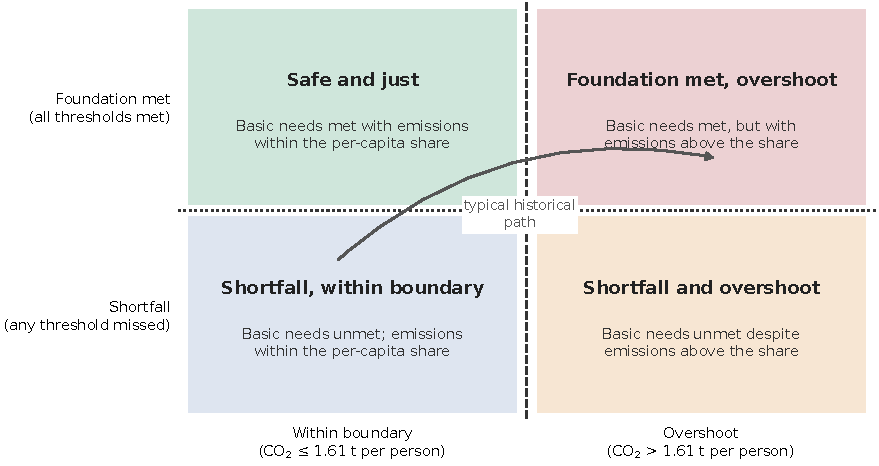
\includegraphics[width=0.8\textwidth]{../figures/fig0_framework.pdf}
\caption{The four configurations of social attainment and climate pressure. The vertical division is the climate boundary (\nBoundary~t \COtwo{} per person per year, consumption-based). The horizontal division is the social foundation (all four social thresholds met). The arrow sketches the path that, as \cref{sec:results} shows, countries have historically followed: from shortfall within the boundary, through overshoot, to meeting the foundation above the boundary.}
\label{fig:framework}
\end{figure}

Two features of this classification deserve emphasis. First, it is defined by fixed thresholds taken from the literature, not by the sample's own distribution. A country's configuration therefore does not depend on how other countries perform, and a change in configuration over time reflects a change in that country's own outcomes or emissions. Second, the classification is deliberately simple. It summarises a complex reality in two binary criteria. It does not show how far a country is from each threshold, so the paper complements it with continuous measures: the attainment ratio of each social indicator and the ratio of emissions to the boundary.

\subsection{The carbon requirement}

The configurations show where countries are. They do not directly show how the relationship between emissions and social attainment has changed. To summarise that relationship, the paper uses the carbon requirement of meeting the social foundation.

The idea is as follows. Across countries in any given year, the probability that a country meets the social foundation rises with its emissions per person, because emissions are associated with energy use, income and infrastructure. This relationship can be summarised by a curve that gives the probability of meeting the foundation at each level of emissions. The carbon requirement is the level of emissions per person at which this curve reaches 50\%. If the curve shifts to the left over time, so that a given probability is reached at lower emissions, the requirement falls. This means meeting the foundation has become less carbon-intensive in the cross-country distribution.

It is important to be clear about what the carbon requirement is and is not.
\begin{itemize}
\item It \emph{is} a descriptive summary of the joint distribution of emissions and social attainment across countries in a given year. It provides a single, interpretable number that can be compared with the climate boundary and tracked over time.
\item It is \emph{not} an estimate of the emissions any particular country needs to meet the foundation. Countries at the same emission level differ widely in their social outcomes, and some meet the foundation at emissions far below the requirement. \Cref{sec:results} shows these ``frontier'' countries explicitly.
\item It is \emph{not} a causal estimate. Emissions are correlated with many other determinants of social outcomes, such as income, institutions, health systems and geography. The requirement does not separate their effects, and a fall in the requirement does not identify why the relationship changed.
\item Its \emph{level} depends on the definition of the social foundation. A more demanding foundation raises the requirement; a less demanding one lowers it. The paper therefore reports the requirement under several definitions and treats its trend and its position relative to the boundary, rather than its exact level, as the robust findings.
\end{itemize}

\subsection{Decoupling and the pace required by the boundary}

For countries above the boundary, the relevant question is not only whether emissions are falling, but whether they are falling fast enough. The boundary implies a destination. A country that emits 8~t per person in 2022 must reduce its emissions by about 5.6\% a year to reach 1.61~t by 2050. A country that cuts its emissions by 1.5\% a year is decoupling in the usual sense, but would take more than a century to arrive. The analysis therefore compares, for each country, the rate at which emissions per person actually changed with the rate required to reach the boundary by 2050. This comparison does not predict future emissions. It measures the gap between the pace of change observed so far and the pace the boundary requires.

\subsection{Expectations}

The literature reviewed in \cref{sec:literature} suggests four expectations, which correspond to the four research questions.

\begin{enumerate}[label=\textbf{E\arabic*.},leftmargin=2.5em]
\item \textbf{Few or no countries in the safe and just space} (RQ1). Based on \citet{oneill2018} and \citet{fanning2022}, few if any countries are expected to meet the social foundation within the climate boundary. Countries reaching the foundation are expected to do so mostly above the boundary.
\item \textbf{A falling carbon requirement} (RQ2). Based on the evidence of a declining carbon intensity of well-being \citep{steinberger2010,jorgenson2014}, the carbon requirement is expected to fall over time. Whether it has fallen to the boundary is an open question.
\item \textbf{Widespread but insufficient decoupling} (RQ3). Based on \citet{haberl2020} and \citet{vogel2023}, absolute decoupling is expected to have become more common, but achieved rates are expected to fall short of those required.
\item \textbf{Persistent configurations} (RQ4). Because energy systems, infrastructure and social institutions change slowly, most countries are expected to remain in the same configuration from one decade to the next. The movements that do occur are expected to run from social shortfall towards the foundation, typically accompanied by rising emissions.
\end{enumerate}
